\section{Auswertung}
\rhead{Auswertung}
\subsection{Simulation El-Niño mit realen Werten}
Der Matlab-Code zur Simulation des El-Niño DDE ist nun vorhanden.
Zur Überprüfung ob die Simulation plausibel ist, wird eine Zeitperiode in der Vergangenheit berechnet.
Ausgewählt zur Simulation wird die Zeitperiode ab September 1995. 
Also werden die Daten von Januar bis September 1995 als History genommen.

Simuliert wird 1 Jahr (Abbildung \ref{fig:sim1}), 3 Jahre (Abbildung \ref{fig:sim3}) und 10 Jahre (Abbildung \ref{fig:sim10}). 
Die Konstanten wurden so verändert, dass das Resultat auf 3 Jahre gut stimmt.
\begin{figure}
	\centering
	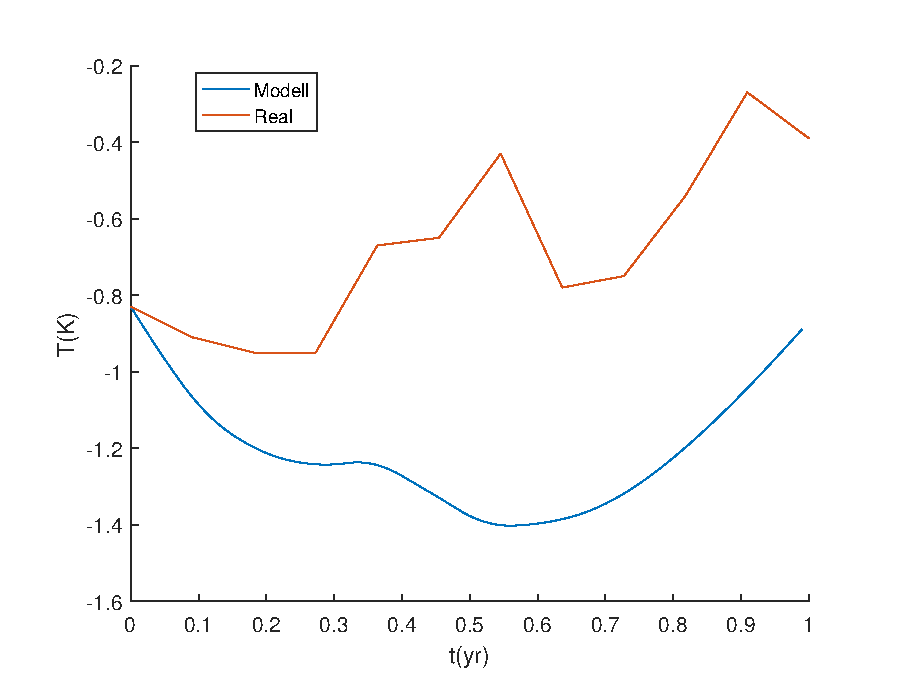
\includegraphics[width=0.66\textwidth,height=0.33\textheight]{verzoegert/inp/figures/sim_1.eps}
	\caption{El-Niño Simulation von 1995-1996 und Vergleich mit realen Daten}
	\label{fig:sim1}
\end{figure}
\begin{figure}
	\centering
	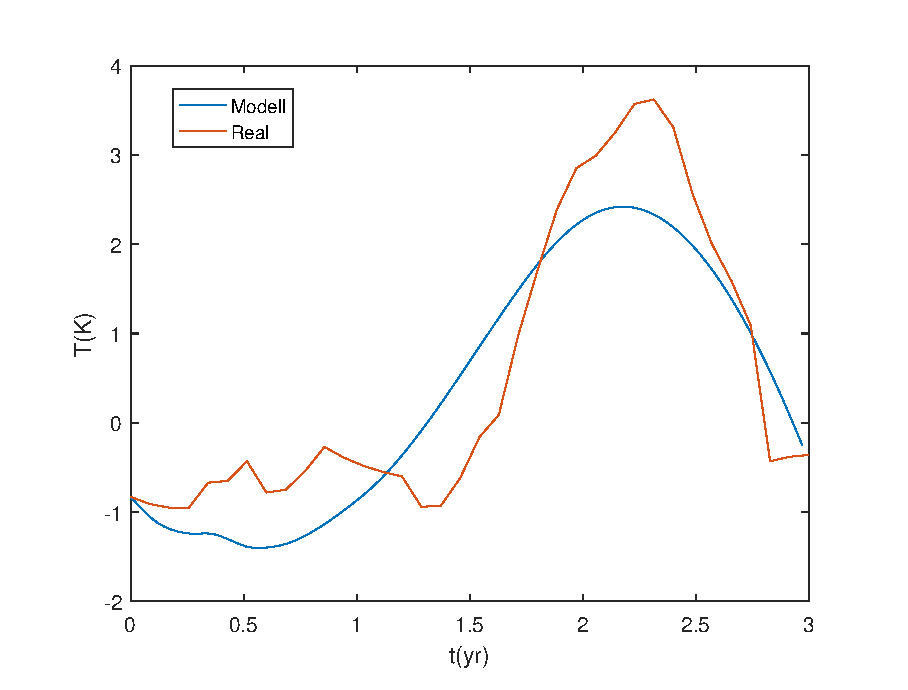
\includegraphics[width=0.66\textwidth,height=0.33\textheight]{verzoegert/inp/figures/sim_3.eps}
	\caption{El-Niño Simulation von 1995-1998 und Vergleich mit realen Daten}
	\label{fig:sim3}
\end{figure}
\begin{figure}
	\centering
	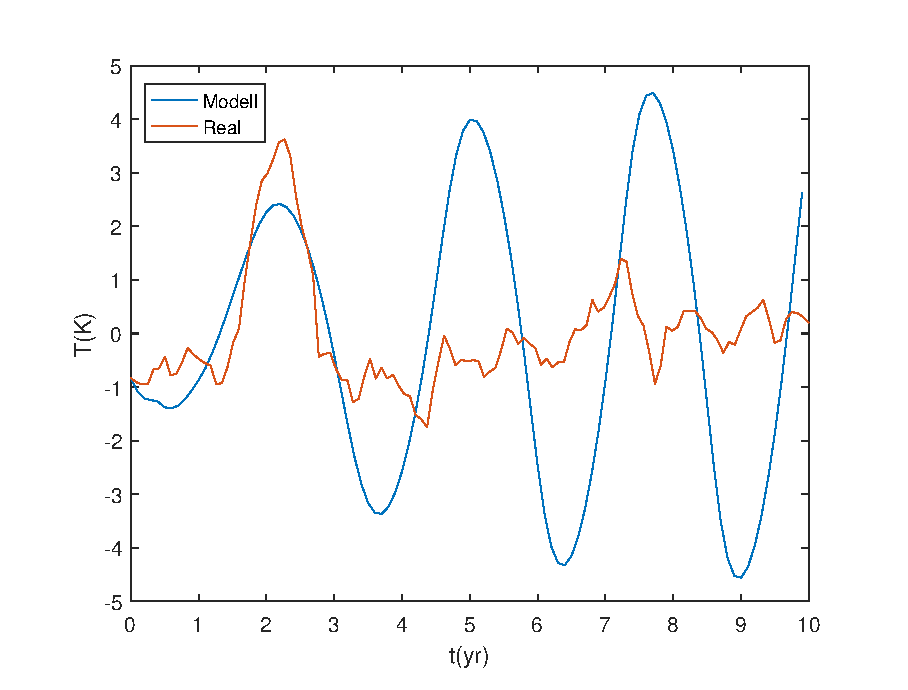
\includegraphics[width=0.66\textwidth,height=0.33\textheight]{verzoegert/inp/figures/sim_10.eps}
	\caption{El-Niño Simulation von 1995-2005 und Vergleich mit realen Daten}
	\label{fig:sim10}
\end{figure}
Mit den richtigen Konstanten lassen sich für kurze Zeiten relativ gute Vorhersagen machen.
Allerdings ist das El-Niño-Phänomen (vgl. Abbildung \ref{fig:elnino}) extrem unkonstant und bräuchte ein komplexeres Modell.
Über längere Zeit versagt das Modell, da es immer zu einer gleichmäßigen Oszillation kommt.

Interessant ist, dass die DDE das kurzfristige Verhalten (1 Jahr, Abbildung \ref{fig:sim1}) richtig berechnet.
Das sieht man an der kurzen Richtungsänderung zwischen 0.3 und 0.4 Jahren.



\subsection{Fazit}
Mit verzögerten Differentialgleichungen können diverse Probleme gelöst werden.
DDEs können analytisch untersucht werden, die Komplexität nimmt allerdings schnell zu.
Eine numerische Simulation ist daher zwingend.
Eine solche Simulation kann relativ einfach erstellt werden und liefert gute Resultate.
Man sollte die Resultate trotzdem genau prüfen, da die Lösungen schnell instabil werden können (vgl. \ref{num:instabil}).

Das Modell zur Modellierung des El-Niño-Phänomens ist sicher noch nicht vollständig.
Es ist aber ein schönes Beispiel einer Anwendung von verzögerten Differentialgleichungen. 